\documentclass[12pt]{beamer}\usepackage[]{graphicx}\usepackage[]{color}
%% maxwidth is the original width if it is less than linewidth
%% otherwise use linewidth (to make sure the graphics do not exceed the margin)
\makeatletter
\def\maxwidth{ %
  \ifdim\Gin@nat@width>\linewidth
    \linewidth
  \else
    \Gin@nat@width
  \fi
}
\makeatother

\definecolor{fgcolor}{rgb}{0.345, 0.345, 0.345}
\newcommand{\hlnum}[1]{\textcolor[rgb]{0.686,0.059,0.569}{#1}}%
\newcommand{\hlstr}[1]{\textcolor[rgb]{0.192,0.494,0.8}{#1}}%
\newcommand{\hlcom}[1]{\textcolor[rgb]{0.678,0.584,0.686}{\textit{#1}}}%
\newcommand{\hlopt}[1]{\textcolor[rgb]{0,0,0}{#1}}%
\newcommand{\hlstd}[1]{\textcolor[rgb]{0.345,0.345,0.345}{#1}}%
\newcommand{\hlkwa}[1]{\textcolor[rgb]{0.161,0.373,0.58}{\textbf{#1}}}%
\newcommand{\hlkwb}[1]{\textcolor[rgb]{0.69,0.353,0.396}{#1}}%
\newcommand{\hlkwc}[1]{\textcolor[rgb]{0.333,0.667,0.333}{#1}}%
\newcommand{\hlkwd}[1]{\textcolor[rgb]{0.737,0.353,0.396}{\textbf{#1}}}%
\let\hlipl\hlkwb

\usepackage{framed}
\makeatletter
\newenvironment{kframe}{%
 \def\at@end@of@kframe{}%
 \ifinner\ifhmode%
  \def\at@end@of@kframe{\end{minipage}}%
  \begin{minipage}{\columnwidth}%
 \fi\fi%
 \def\FrameCommand##1{\hskip\@totalleftmargin \hskip-\fboxsep
 \colorbox{shadecolor}{##1}\hskip-\fboxsep
     % There is no \\@totalrightmargin, so:
     \hskip-\linewidth \hskip-\@totalleftmargin \hskip\columnwidth}%
 \MakeFramed {\advance\hsize-\width
   \@totalleftmargin\z@ \linewidth\hsize
   \@setminipage}}%
 {\par\unskip\endMakeFramed%
 \at@end@of@kframe}
\makeatother

\definecolor{shadecolor}{rgb}{.97, .97, .97}
\definecolor{messagecolor}{rgb}{0, 0, 0}
\definecolor{warningcolor}{rgb}{1, 0, 1}
\definecolor{errorcolor}{rgb}{1, 0, 0}
\newenvironment{knitrout}{}{} % an empty environment to be redefined in TeX

\usepackage{alltt}
\usepackage{graphicx}
\usepackage{amsmath}
\usepackage{tikz}
\setbeameroption{hide notes}
\setbeamertemplate{note page}[plain]
\usepackage{listings}

% get rid of junk
\usetheme{default}
\usefonttheme[onlymath]{serif}
\beamertemplatenavigationsymbolsempty
\hypersetup{pdfpagemode=UseNone} % don't show bookmarks on initial view

% named colors
\definecolor{offwhite}{RGB}{255,250,240}
\definecolor{gray}{RGB}{155,155,155}

\ifx\notescolors\undefined % slides

  \definecolor{foreground}{RGB}{80,80,80}
  \definecolor{background}{RGB}{255,255,255}
  \definecolor{title}{RGB}{255,199,0}
  \definecolor{subtitle}{RGB}{89,132,212}
  \definecolor{hilit}{RGB}{248,117,79}
  \definecolor{vhilit}{RGB}{255,111,207}
  \definecolor{lolit}{RGB}{200,200,200}
  \definecolor{lit}{RGB}{255,199,0}
  \definecolor{mdlit}{RGB}{89,132,212}
  \definecolor{link}{RGB}{248,117,79}

\else % notes
  \definecolor{background}{RGB}{255,255,255}
  \definecolor{foreground}{RGB}{24,24,24}
  \definecolor{title}{RGB}{27,94,134}
  \definecolor{subtitle}{RGB}{22,175,124}
  \definecolor{hilit}{RGB}{122,0,128}
  \definecolor{vhilit}{RGB}{255,0,128}
  \definecolor{lolit}{RGB}{95,95,95}
\fi
\definecolor{nhilit}{RGB}{128,0,128}  % hilit color in notes
\definecolor{nvhilit}{RGB}{255,0,128} % vhilit for notes

\newcommand{\hilit}{\color{hilit}}
\newcommand{\vhilit}{\color{vhilit}}
\newcommand{\nhilit}{\color{nhilit}}
\newcommand{\nvhilit}{\color{nvhilit}}
\newcommand{\lit}{\color{lit}}
\newcommand{\mdlit}{\color{mdlit}}
\newcommand{\lolit}{\color{lolit}}

% use those colors
\setbeamercolor{titlelike}{fg=title}
\setbeamercolor{subtitle}{fg=subtitle}
\setbeamercolor{frametitle}{fg=gray}
\setbeamercolor{structure}{fg=subtitle}
\setbeamercolor{institute}{fg=lolit}
\setbeamercolor{normal text}{fg=foreground,bg=background}
%\setbeamercolor{item}{fg=foreground} % color of bullets
%\setbeamercolor{subitem}{fg=hilit}
%\setbeamercolor{itemize/enumerate subbody}{fg=lolit}
\setbeamertemplate{itemize subitem}{{\textendash}}
\setbeamerfont{itemize/enumerate subbody}{size=\footnotesize}
\setbeamerfont{itemize/enumerate subitem}{size=\footnotesize}

% center title of slides
\setbeamertemplate{blocks}[rounded]
\setbeamertemplate{frametitle}[default][center]
% margins
\setbeamersize{text margin left=25pt,text margin right=25pt}

% page number
\setbeamertemplate{footline}{%
    \raisebox{5pt}{\makebox[\paperwidth]{\hfill\makebox[20pt]{\lolit
          \scriptsize\insertframenumber}}}\hspace*{5pt}}

% add a bit of space at the top of the notes page
\addtobeamertemplate{note page}{\setlength{\parskip}{12pt}}

% default link color
\hypersetup{colorlinks, urlcolor={link}}

\ifx\notescolors\undefined % slides
  % set up listing environment
  \lstset{language=bash,
          basicstyle=\ttfamily\scriptsize,
          frame=single,
          commentstyle=,
          backgroundcolor=\color{darkgray},
          showspaces=false,
          showstringspaces=false
          }
\else % notes
  \lstset{language=bash,
          basicstyle=\ttfamily\scriptsize,
          frame=single,
          commentstyle=,
          backgroundcolor=\color{offwhite},
          showspaces=false,
          showstringspaces=false
          }
\fi

% a few macros
\newcommand{\code}[1]{\texttt{#1}}
\newcommand{\hicode}[1]{{\hilit \texttt{#1}}}
\newcommand{\bb}[1]{\begin{block}{#1}}
\newcommand{\eb}{\end{block}}
\newcommand{\bi}{\begin{itemize}}
%\newcommand{\bbi}{\vspace{24pt} \begin{itemize} \itemsep8pt}
\newcommand{\bbi}{\vspace{4pt} \begin{itemize} \itemsep8pt}
\newcommand{\ei}{\end{itemize}}
\newcommand{\bv}{\begin{verbatim}}
\newcommand{\ev}{\end{verbatim}}
\newcommand{\ig}{\includegraphics}
\newcommand{\subt}[1]{{\footnotesize \color{subtitle} {#1}}}
\newcommand{\ttsm}{\tt \small}
\newcommand{\ttfn}{\tt \footnotesize}
\newcommand{\figh}[2]{\centerline{\includegraphics[height=#2\textheight]{#1}}}
\newcommand{\figw}[2]{\centerline{\includegraphics[width=#2\textwidth]{#1}}}



%------------------------------------------------
% end of header
%------------------------------------------------

\title{Random Numbers}
\subtitle{STAT 133}
\author{\href{http://www.gastonsanchez.com}{Gaston Sanchez}}
\institute{\href{https://github.com/ucb-stat133/stat133-fall-2016}{\tt \scriptsize \color{foreground} github.com/ucb-stat133/stat133-fall-2016}}
\date{}
\IfFileExists{upquote.sty}{\usepackage{upquote}}{}
\begin{document}


{
  \setbeamertemplate{footline}{} % no page number here
  \frame{
    \titlepage
  } 
}

%------------------------------------------------

\begin{frame}
\begin{center}
\Huge{\hilit{Random Numbers in R}}
\end{center}
\end{frame}

%------------------------------------------------

\begin{frame}
\frametitle{Generating Random Numbers}

\Large Generation of random numbers is at the heart of many statistical methods

\end{frame}

%------------------------------------------------

\begin{frame}
\frametitle{Use of Random Numbers}

\bb{Some uses of random numbers}
\bbi
  \item Sampling procedures
  \item Simulation studies of stochastic processes
  \item Analytically intractable mathematical expressions
  \item Simulation of a population distribution by resampling from a given sample from that population
  \item More general: Simulation, Monte Carlo, Resampling
\ei
\eb

\end{frame}

%------------------------------------------------

\begin{frame}
\frametitle{Random Samples}

\bi
  \item Many statistical methods rely on random samples:
  \bi
    \item Sampling techniques
    \item Design of experiments
    \item Surveys
  \ei
  \item Hence, we need a source of random numbers
  \item Before computers, statisticians used \textit{tables of random numbers}
  \item Now we use computers to generate ``random'' numbers
  \item The random sampling required in most analyses is usually done by the computer
\ei

\end{frame}

%------------------------------------------------

\begin{frame}
\frametitle{Generating Random Numbers}

\bbi
  \item We cannot generate truly random numbers on a computer
  \item Instead, we generate \textbf{pseudo-random} numbers
  \item i.e. numbers that have the appearance of random numbers
  \item they \textit{seem} to be randomly drawn from some known distribution
  \item There are many methods that have been proposed to generate pseudo-random numbers
\ei

\end{frame}

%------------------------------------------------

\begin{frame}
\frametitle{Generating Random Numbers}

\Large A very important advantage of using pseudo-random numbers is that, because they are deterministic, they can be reproduced (i.e. repeated)

\end{frame}

%------------------------------------------------

\begin{frame}[fragile]
\frametitle{Multiple Recursion}

\bbi
  \item Generate a sequence of numbers in a manner that appears to be random
  \item Use a deterministic generator that yields numbers recursively (in a fixed sequence)
  \item The previous $k$ numbers determine the next one
\ei
$$
x_i = f(x_{i-1}, \dots, x_{i-k})
$$

\end{frame}

%------------------------------------------------

\begin{frame}
\frametitle{Simple Congruential Generator}

\bi
  \item Congruential generators were the first reasonable class of pseudo-random number generators
  \item The congruential method uses modular arithmetic to generate ``random'' numbers
\ei

\end{frame}

%------------------------------------------------

\begin{frame}
\frametitle{Ingredients}

\bi
  \item An integer $m$
  \item An integer $a$ such that $a < m$
  \item A starting integer $x_0$ (a.k.a. \textit{seed})
\ei

\end{frame}

%------------------------------------------------

\begin{frame}[fragile]
\frametitle{Simple Congruential Generator}

The first number is obtained as: \\
$
x_{1} = (a \times x_{0}) \text{ mod } m
$

\bigskip
The rest of the pseudorandom numbers are generated as:\\
$
x_{n+1} = (a \times x_{n}) \text{ mod } m
$
\end{frame}

%------------------------------------------------

\begin{frame}[fragile]
\frametitle{Simple Congruential Generator}

For example if we take $m = 64$, and $a = 3$, then for $x_0 = 17$ we have:

\begin{align*} 
x_1 &= (3 \times 17) \text{ mod } 64 = 51 \\ 
x_2 &= (3 \times 51) \text{ mod } 64 = 25 \\
x_3 &= (3 \times 25) \text{ mod } 64 = 11 \\
x_4 &= (3 \times 11) \text{ mod } 64 = 33 \\ 
x_5 &= (3 \times 33) \text{ mod } 64 = 35 \\
x_6 &= (3 \times 35) \text{ mod } 64 = 41 \\
\vdots \\
\end{align*}

\end{frame}

%------------------------------------------------

\begin{frame}[fragile]
\frametitle{Congruential algorithm}

\begin{knitrout}\footnotesize
\definecolor{shadecolor}{rgb}{0.969, 0.969, 0.969}\color{fgcolor}\begin{kframe}
\begin{alltt}
\hlstd{a} \hlkwb{<-} \hlnum{3}\hlstd{;  m} \hlkwb{<-} \hlnum{64}\hlstd{;  seed} \hlkwb{<-} \hlnum{17}

\hlstd{x} \hlkwb{<-} \hlkwd{numeric}\hlstd{(}\hlnum{20}\hlstd{)}

\hlstd{x[}\hlnum{1}\hlstd{]} \hlkwb{<-} \hlstd{(a} \hlopt{*} \hlstd{seed)} \hlopt \hlstd{m}

\hlkwa{for} \hlstd{(i} \hlkwa{in} \hlnum{2}\hlopt{:}\hlnum{20}\hlstd{) \{}
  \hlstd{x[i]} \hlkwb{<-} \hlstd{(a} \hlopt{*} \hlstd{x[i}\hlopt{-}\hlnum{1}\hlstd{])} \hlopt \hlstd{m}
\hlstd{\}}

\hlstd{x[}\hlnum{1}\hlopt{:}\hlnum{16}\hlstd{]; x[}\hlnum{17}\hlopt{:}\hlnum{20}\hlstd{]}
\end{alltt}
\begin{verbatim}
##  [1] 51 25 11 33 35 41 59 49 19 57 43  1  3  9 27 17
## [1] 51 25 11 33
\end{verbatim}
\end{kframe}
\end{knitrout}

\end{frame}

%------------------------------------------------

\begin{frame}[fragile]
\frametitle{Congruential algorithm}
\begin{knitrout}\footnotesize
\definecolor{shadecolor}{rgb}{0.969, 0.969, 0.969}\color{fgcolor}\begin{kframe}
\begin{alltt}
\hlstd{cong} \hlkwb{<-} \hlkwa{function}\hlstd{(}\hlkwc{n}\hlstd{,} \hlkwc{a} \hlstd{=} \hlnum{69069}\hlstd{,} \hlkwc{m} \hlstd{=} \hlnum{2}\hlopt{^}\hlnum{32}\hlstd{,} \hlkwc{seed} \hlstd{=} \hlnum{17}\hlstd{) \{}
  \hlstd{x} \hlkwb{<-} \hlkwd{numeric}\hlstd{(n)}
  \hlstd{x[}\hlnum{1}\hlstd{]} \hlkwb{<-} \hlstd{(a} \hlopt{*} \hlstd{seed)} \hlopt \hlstd{m}
  \hlkwa{for} \hlstd{(i} \hlkwa{in} \hlnum{2}\hlopt{:}\hlstd{n) \{}
    \hlstd{x[i]} \hlkwb{<-} \hlstd{(a} \hlopt{*} \hlstd{x[i}\hlopt{-}\hlnum{1}\hlstd{])} \hlopt \hlstd{m}
  \hlstd{\}}
  \hlstd{x}
\hlstd{\}}

\hlstd{y} \hlkwb{<-} \hlkwd{cong}\hlstd{(}\hlnum{20}\hlstd{,} \hlkwc{a} \hlstd{=} \hlnum{3}\hlstd{,} \hlkwc{m} \hlstd{=} \hlnum{64}\hlstd{,} \hlkwc{seed} \hlstd{=} \hlnum{17}\hlstd{)}
\end{alltt}
\end{kframe}
\end{knitrout}

\end{frame}

%------------------------------------------------

\begin{frame}[fragile]
\frametitle{Congruential algorithm}
\begin{knitrout}\tiny
\definecolor{shadecolor}{rgb}{0.969, 0.969, 0.969}\color{fgcolor}\begin{kframe}
\begin{alltt}
\hlkwd{plot}\hlstd{(y[}\hlnum{1}\hlopt{:}\hlstd{(n}\hlopt{-}\hlnum{1}\hlstd{)], y[}\hlnum{2}\hlopt{:}\hlstd{n],} \hlkwc{pch} \hlstd{=} \hlnum{19}\hlstd{,}
     \hlkwc{xlab} \hlstd{=} \hlstr{'current value'}\hlstd{,} \hlkwc{ylab} \hlstd{=} \hlstr{'next value'}\hlstd{)}
\end{alltt}
\end{kframe}

{\centering 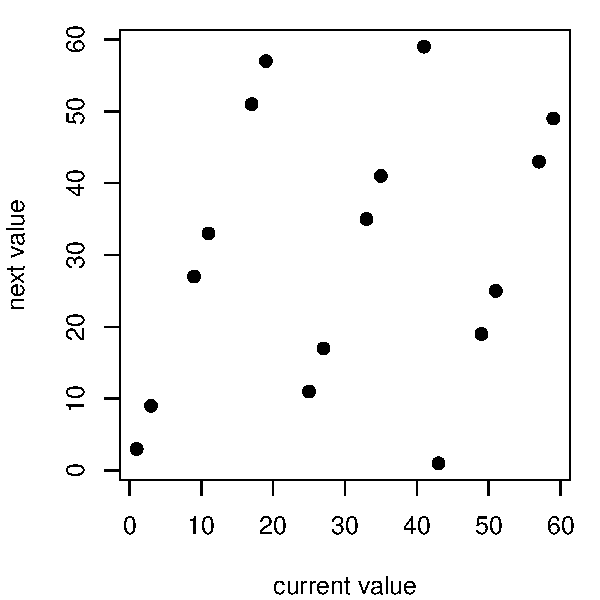
\includegraphics[width=.6\linewidth,height=.6\linewidth]{figure/unnamed-chunk-3-1} 

}



\end{knitrout}

\end{frame}

%------------------------------------------------

\begin{frame}[fragile]

\code{cong(n, a = 69069, m = 2\string^32, seed = 17)}
\begin{knitrout}\footnotesize
\definecolor{shadecolor}{rgb}{0.969, 0.969, 0.969}\color{fgcolor}

{\centering 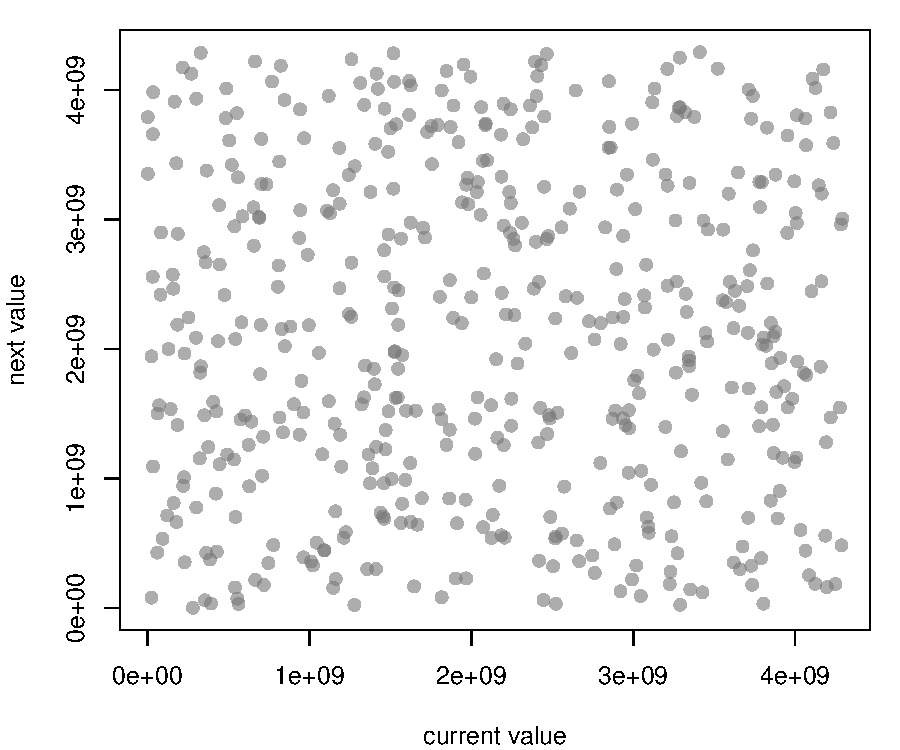
\includegraphics[width=.8\linewidth,height=.65\linewidth]{figure/unnamed-chunk-4-1} 

}



\end{knitrout}

\end{frame}

%------------------------------------------------

\begin{frame}
\frametitle{Ingredients}

\bi
  \item $m$ is the modulus ($0 < m$)
  \item $a$ is the multiplier ($0 < a < m$)
  \item $x_0$ is the seed ($0 \leq x_0 \leq m$)
\ei

\bigskip
The period length of a Random Generator Number is at most $m$, and for some choices of $a$ much less than that.

\end{frame}

%------------------------------------------------

\begin{frame}
\frametitle{About the seed}

\bi
  \item You can reproduce your simulation results by controlling the seed
  \item {\hilit \code{set.seed()}} allows to do this
  \item Every time you perform simulation studies indicate the random number generator and the seed that was used
\ei

\end{frame}

%------------------------------------------------

\begin{frame}[fragile]
\frametitle{About the seed}

\begin{knitrout}\footnotesize
\definecolor{shadecolor}{rgb}{0.969, 0.969, 0.969}\color{fgcolor}\begin{kframe}
\begin{alltt}
\hlcom{# set the seed}
\hlkwd{set.seed}\hlstd{(}\hlnum{69069}\hlstd{)}

\hlkwd{runif}\hlstd{(}\hlnum{3}\hlstd{)}  \hlcom{# call the uniform RNG}
\end{alltt}
\begin{verbatim}
## [1] 0.1648855 0.9564664 0.3345479
\end{verbatim}
\begin{alltt}
\hlkwd{runif}\hlstd{(}\hlnum{3}\hlstd{)}  \hlcom{# call runif() again}
\end{alltt}
\begin{verbatim}
## [1] 0.01109596 0.18654873 0.94657805
\end{verbatim}
\begin{alltt}
\hlcom{# set the seed back to 69069}
\hlkwd{set.seed}\hlstd{(}\hlnum{69069}\hlstd{)}
\hlkwd{runif}\hlstd{(}\hlnum{3}\hlstd{)}
\end{alltt}
\begin{verbatim}
## [1] 0.1648855 0.9564664 0.3345479
\end{verbatim}
\end{kframe}
\end{knitrout}

\end{frame}

%------------------------------------------------

\begin{frame}
\frametitle{Simple Congruential Generator}

We can use a congruential algorithm to generate uniform numbers

\bigskip
We'll describe one of the simplest methods for simulating independent uniform random variables on the interaval [0, 1]

\end{frame}

%------------------------------------------------

\begin{frame}
\frametitle{Generating Uniform Numbers}

The generator proceeds as follows
\begin{align*} 
x_1 &= (a x_0) \text{ mod } m \\
u_1 &= x_1 / m \\
\end{align*}

$u_1$ is the first pseudo-random number, taking some value between 0 and 1.

\end{frame}

%------------------------------------------------

\begin{frame}
\frametitle{Ingredients}

The second pseudorandom number is obtained as:
\begin{align*} 
x_2 &= (a x_1) \text{ mod } m \\
u_2 &= x_2 / m \\
\end{align*}

$u_2$ is another pseudorandom number.

\end{frame}

%------------------------------------------------

\begin{frame}
\frametitle{Generating Uniform Numbers}

\bi
  \item If $m$ and $a$ are chosen properly, it is difficult to predict the value $u_2$ given $u_1$
  \item For most practical purposes $u_2$ is approximately independent of $u_1$
\ei

\end{frame}

%------------------------------------------------

\begin{frame}[fragile]
\frametitle{Simple Congruential Generator}

For example if we take $m = 7$, and $a = 3$, then for $x_0 = 2$ we have:

\begin{align*} 
x_1 &= (3 \times 2) \text{ mod } 7 = 6, \quad u_1 = 0.857 \\ 
x_2 &= (3 \times 6) \text{ mod } 7 = 4, \quad u_2 = 0.571 \\
x_3 &= (3 \times 4) \text{ mod } 7 = 5, \quad u_3 = 0.714 \\
x_4 &= (3 \times 5) \text{ mod } 7 = 1, \quad u_4 = 0.143 \\ 
x_5 &= (3 \times 1) \text{ mod } 7 = 3, \quad u_5 = 0.429 \\
x_6 &= (3 \times 3) \text{ mod } 7 = 2, \quad u_6 = 0.286 \\
\vdots \\
\end{align*}

\end{frame}

%------------------------------------------------

\begin{frame}
\frametitle{Random Numbers in R}

\bb{R uses a pseudo random number generator}
\bi
  \item It starts with a \textbf{seed} and an \textbf{algorithm} (i.e. function)
  \item The seed is plugged into the algorithm and a number is returned
  \item That number is then plugged into the algorithm and the next number is created
  \item The algorithm is such that the produced numbers behave like random numbers
\ei
\eb

\end{frame}

%------------------------------------------------

\begin{frame}[fragile]
\frametitle{RNG functions in R}

\begin{center}
 \begin{tabular}{l l}
 \hline
  Function & Description \\
  \hline
  \code{runif()} & Uniform \\  
  \code{rbinom()} & Binomial \\
  \code{rmultinom()} & Multinomial \\  
  \code{rnbinom()} & Negative binomial \\  
  \code{rpois()} & Poisson \\  
  \code{rnorm()} & Normal \\
  \code{rbeta()} & Beta \\  
  \code{rgamma()} & Gamma \\
  \code{rchisq()} & Chi-squared \\
  \code{rcauchy()} & Cauchy \\  
  \hline
 \end{tabular}
\end{center}

See more info: \code{?Distributions}

\end{frame}

%------------------------------------------------

\begin{frame}
\frametitle{Random Number Functions}

{\hilit \code{runif(n, min = 0, max = 1)}} sample from the uniform distribution on the interval (0,1)

\bigskip
The chance the value drawn is:
\bi
  \item between 0 and 1/3 has chance 1/3
  \item between 1/3 and 1/2 has chance 1/6
  \item between 9/10 and 1 has chance 1/10
\ei

\end{frame}

%------------------------------------------------

\begin{frame}
\frametitle{Random Number Functions}

{\hilit \code{rnorm(n, mean = 0, sd = 1)}} sample from the normal distribution with center = \code{mean} and spread = \code{sd}

\pause
\bigskip
{\hilit \code{rbinom(n, size, prob)}} sample from the binomial distribution with number of trials = \code{size} and chance of success = \code{prob}

\end{frame}

%------------------------------------------------

\begin{frame}
\begin{center}
\Huge{\hilit{Bootstrapping}}
\end{center}
\end{frame}

%------------------------------------------------

\begin{frame}
\frametitle{Let's Generalize}

\bbi
  \item A \textbf{statistic} is just a function of a random sample
  \item Statistics are used as estimators of quantities of interest about the distribution, called \textbf{parameters}
  \item Statistics are random variables
  \item Parameters are NOT random variables
\ei

\end{frame}

%------------------------------------------------

\begin{frame}
\frametitle{Let's Generalize}

\bbi
  \item In simple cases, we can study the \textit{sampling distribution} of the statistic analytically
  \item e.g. we can prove under mild conditions that the distribution of the sample proportion is close to normal for large sample sizes
  \item In more complicated cases we can turn to simulation
\ei

\end{frame}

%------------------------------------------------

\begin{frame}
\frametitle{Sampling Distributions}

\bbi
  \item In our example $X_1, X_2, \dots, X_n$ are independent observations from the same distribution
  \item The distribution has center (mean value) $\mu$ and spread (standard deviation) $\sigma$
  \item e.g. interest in the distribution of $median(X_1, X_2, \dots, X_n)$
  \item We take many samples of size $n$, and study the behavior of the sample medians
\ei

\end{frame}

%------------------------------------------------

\begin{frame}
\frametitle{Some Limitations}

\bi
  \item Consider \textit{t-test} procedures for inference about means
  \item Most classical methods rest on the use of Normal Distributions
  \item However, most real data are not Normal
  \item We cannot use $t$ confidence intervals for strongly skewed data (unless samples are large)
  \item What about inference for a \textit{ratio} of means? (no simple traditional inference)
\ei

\end{frame}

%------------------------------------------------

\begin{frame}
\frametitle{Fundamental Reasoning}

\bi
  \item Apply computer power to relax some of the conditions needed in traditional tests
  \item Have tools to do inference in new settings
  \item What would happen if we applied this method many times?
\ei

\end{frame}

%------------------------------------------------

\begin{frame}
\frametitle{Bootstrap Idea}

\bi
  \item Statistical inference is based on the sampling distributions of sample statistics
  \item A sampling distribution is based on many random samples from the population
  \item The bootstrap is a way of finding the sampling distribution (approximately)
\ei

\end{frame}

%------------------------------------------------

\begin{frame}[fragile]
\frametitle{Bootstrap Samples}

\begin{knitrout}\footnotesize
\definecolor{shadecolor}{rgb}{0.969, 0.969, 0.969}\color{fgcolor}\begin{kframe}
\begin{alltt}
\hlstd{x} \hlkwb{<-} \hlkwd{c}\hlstd{(}\hlnum{3.15}\hlstd{,} \hlnum{0}\hlstd{,} \hlnum{1.58}\hlstd{,} \hlnum{19.65}\hlstd{,} \hlnum{0.23}\hlstd{,} \hlnum{2.21}\hlstd{)}
\hlkwd{mean}\hlstd{(x)}
\end{alltt}
\begin{verbatim}
## [1] 4.47
\end{verbatim}
\end{kframe}
\end{knitrout}

\pause
\begin{knitrout}\footnotesize
\definecolor{shadecolor}{rgb}{0.969, 0.969, 0.969}\color{fgcolor}\begin{kframe}
\begin{alltt}
\hlstd{(x1} \hlkwb{<-} \hlkwd{sample}\hlstd{(x,} \hlkwc{size} \hlstd{=} \hlnum{6}\hlstd{,} \hlkwc{replace} \hlstd{=} \hlnum{TRUE}\hlstd{))}
\end{alltt}
\begin{verbatim}
## [1]  3.15  0.00  2.21  3.15 19.65  0.00
\end{verbatim}
\begin{alltt}
\hlkwd{mean}\hlstd{(x1)}
\end{alltt}
\begin{verbatim}
## [1] 4.693333
\end{verbatim}
\end{kframe}
\end{knitrout}

\end{frame}

%------------------------------------------------

\begin{frame}[fragile]
\frametitle{Bootstrap Samples}

\begin{knitrout}\footnotesize
\definecolor{shadecolor}{rgb}{0.969, 0.969, 0.969}\color{fgcolor}\begin{kframe}
\begin{alltt}
\hlstd{(x2} \hlkwb{<-} \hlkwd{sample}\hlstd{(x,} \hlkwc{size} \hlstd{=} \hlnum{6}\hlstd{,} \hlkwc{replace} \hlstd{=} \hlnum{TRUE}\hlstd{))}
\end{alltt}
\begin{verbatim}
## [1] 3.15 2.21 3.15 1.58 1.58 1.58
\end{verbatim}
\begin{alltt}
\hlkwd{mean}\hlstd{(x2)}
\end{alltt}
\begin{verbatim}
## [1] 2.208333
\end{verbatim}
\begin{alltt}
\hlstd{(x3} \hlkwb{<-} \hlkwd{sample}\hlstd{(x,} \hlkwc{size} \hlstd{=} \hlnum{6}\hlstd{,} \hlkwc{replace} \hlstd{=} \hlnum{TRUE}\hlstd{))}
\end{alltt}
\begin{verbatim}
## [1]  1.58  2.21  0.00  0.23 19.65  1.58
\end{verbatim}
\begin{alltt}
\hlkwd{mean}\hlstd{(x3)}
\end{alltt}
\begin{verbatim}
## [1] 4.208333
\end{verbatim}
\end{kframe}
\end{knitrout}

\end{frame}

%------------------------------------------------

\begin{frame}
\frametitle{Procedure for Bootstrapping}

\bbi
  \item Repeatedly sampling \textbf{with replacement} from a random sample
  \item Each bootstrap sample is the same size as the original sample
  \item Calculate the statisc of interest (e.g. mean, median, sd)
  \item Draw hundreds or thousands of samples
  \item Obtain a bootstrap distribution
\ei

\end{frame}

%------------------------------------------------

\begin{frame}[fragile]
\frametitle{Bootstrap Samples}

\begin{knitrout}\footnotesize
\definecolor{shadecolor}{rgb}{0.969, 0.969, 0.969}\color{fgcolor}\begin{kframe}
\begin{alltt}
\hlstd{bootstrap} \hlkwb{<-} \hlkwd{numeric}\hlstd{(}\hlnum{1000}\hlstd{)}

\hlkwa{for} \hlstd{(b} \hlkwa{in} \hlnum{1}\hlopt{:}\hlnum{1000}\hlstd{) \{}
  \hlstd{boot_sample} \hlkwb{<-} \hlkwd{sample}\hlstd{(x,} \hlkwc{size} \hlstd{=} \hlnum{6}\hlstd{,} \hlkwc{replace} \hlstd{=} \hlnum{TRUE}\hlstd{)}
  \hlstd{bootstrap[b]} \hlkwb{<-} \hlkwd{mean}\hlstd{(boot_sample)}
\hlstd{\}}
\end{alltt}
\end{kframe}
\end{knitrout}

\end{frame}

%------------------------------------------------

\begin{frame}[fragile]
\frametitle{Bootstrap Distribution}
\begin{knitrout}\tiny
\definecolor{shadecolor}{rgb}{0.969, 0.969, 0.969}\color{fgcolor}\begin{kframe}
\begin{alltt}
\hlkwd{hist}\hlstd{(bootstrap,} \hlkwc{col} \hlstd{=} \hlstr{'gray70'}\hlstd{,} \hlkwc{las} \hlstd{=} \hlnum{1}\hlstd{)}
\end{alltt}
\end{kframe}

{\centering 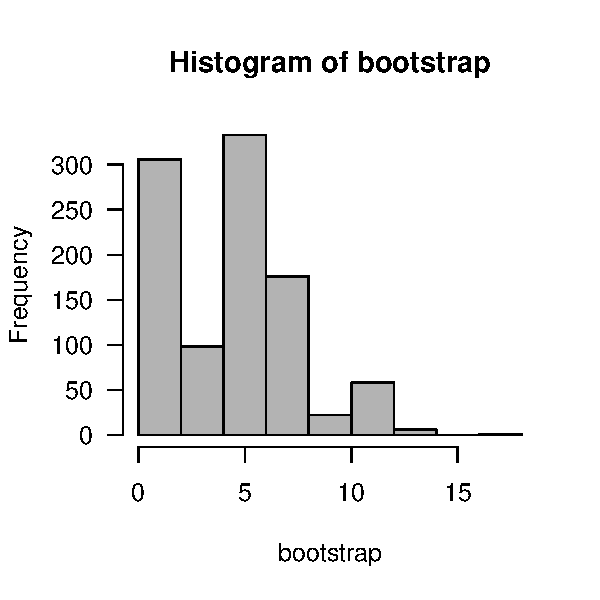
\includegraphics[width=.6\linewidth,height=.6\linewidth]{figure/unnamed-chunk-10-1} 

}



\end{knitrout}

\end{frame}

%------------------------------------------------

\begin{frame}
\frametitle{How does Bootstrapping work?}

\bbi
  \item We are not using the resamples as if they were real data
  \item Bootstrap samples is not a substitute to gather more data to improve accuracy
  \item The bootstrap idea is to use the resample statistics to estimate how the sample statistic varies from the studied random sample
  \item The bootstrap distribution approximates the sampling distribution of the statistic
\ei

\end{frame}

%------------------------------------------------

\begin{frame}
\frametitle{Bootstrap samples}

\bb{Computing the bootstrap distribution implies}
\bbi
  \item Calulate the statistic for each sample
  \item The distribution of these resample statistics is the bootstrap distribution
  \item A bootstrap sample is the same size as the original random sample
\ei
\eb

\end{frame}

%------------------------------------------------

\begin{frame}
\begin{center}
\Huge{\hilit{Another Example}}
\end{center}
\end{frame}

%------------------------------------------------

\begin{frame}[fragile]
\frametitle{Bootstrap resampling}

\begin{knitrout}\footnotesize
\definecolor{shadecolor}{rgb}{0.969, 0.969, 0.969}\color{fgcolor}\begin{kframe}
\begin{alltt}
\hlcom{# Iris Virginica subset (the "population")}
\hlstd{virginica} \hlkwb{<-} \hlkwd{subset}\hlstd{(iris, Species} \hlopt{==} \hlstr{'virginica'}\hlstd{)}

\hlcom{# random sample of Petal.Length (size = 5)}
\hlkwd{set.seed}\hlstd{(}\hlnum{7359}\hlstd{)}
\hlstd{rand_sample} \hlkwb{<-} \hlkwd{sample}\hlstd{(virginica}\hlopt{$}\hlstd{Petal.Length,} \hlkwc{size} \hlstd{=} \hlnum{5}\hlstd{)}
\hlstd{rand_sample}
\end{alltt}
\begin{verbatim}
## [1] 5.1 5.6 5.8 5.7 5.8
\end{verbatim}
\end{kframe}
\end{knitrout}

\end{frame}

%------------------------------------------------

\begin{frame}[fragile]
\frametitle{Bootstrap resampling}

\begin{knitrout}\footnotesize
\definecolor{shadecolor}{rgb}{0.969, 0.969, 0.969}\color{fgcolor}\begin{kframe}
\begin{alltt}
\hlcom{# create 500 bootstrap samples of size 5 with replacement}
\hlstd{resamples} \hlkwb{<-} \hlnum{500}
\hlstd{n} \hlkwb{<-} \hlkwd{length}\hlstd{(rand_sample)}

\hlstd{boot_stats} \hlkwb{<-} \hlkwd{numeric}\hlstd{(resamples)}

\hlkwa{for} \hlstd{(i} \hlkwa{in} \hlnum{1}\hlopt{:}\hlstd{resamples) \{}
  \hlstd{boot_sample} \hlkwb{<-} \hlkwd{sample}\hlstd{(rand_sample,} \hlkwc{size} \hlstd{= n,} \hlkwc{replace} \hlstd{=} \hlnum{TRUE}\hlstd{)}
  \hlstd{boot_stats[i]} \hlkwb{<-} \hlkwd{mean}\hlstd{(boot_sample)}
\hlstd{\}}
\end{alltt}
\end{kframe}
\end{knitrout}

\end{frame}

%------------------------------------------------

\begin{frame}[fragile]
\frametitle{Bootstrap resampling}

\begin{knitrout}\footnotesize
\definecolor{shadecolor}{rgb}{0.969, 0.969, 0.969}\color{fgcolor}\begin{kframe}
\begin{alltt}
\hlcom{# "population" mean }
\hlkwd{mean}\hlstd{(virginica}\hlopt{$}\hlstd{Petal.Length)}
\end{alltt}
\begin{verbatim}
## [1] 5.552
\end{verbatim}
\begin{alltt}
\hlcom{# bootstrap mean}
\hlkwd{mean}\hlstd{(boot_stats)}
\end{alltt}
\begin{verbatim}
## [1] 5.60028
\end{verbatim}
\end{kframe}
\end{knitrout}

\end{frame}

%------------------------------------------------

\begin{frame}[fragile]
\frametitle{Bootstrap Distribution}

\begin{knitrout}\footnotesize
\definecolor{shadecolor}{rgb}{0.969, 0.969, 0.969}\color{fgcolor}

{\centering 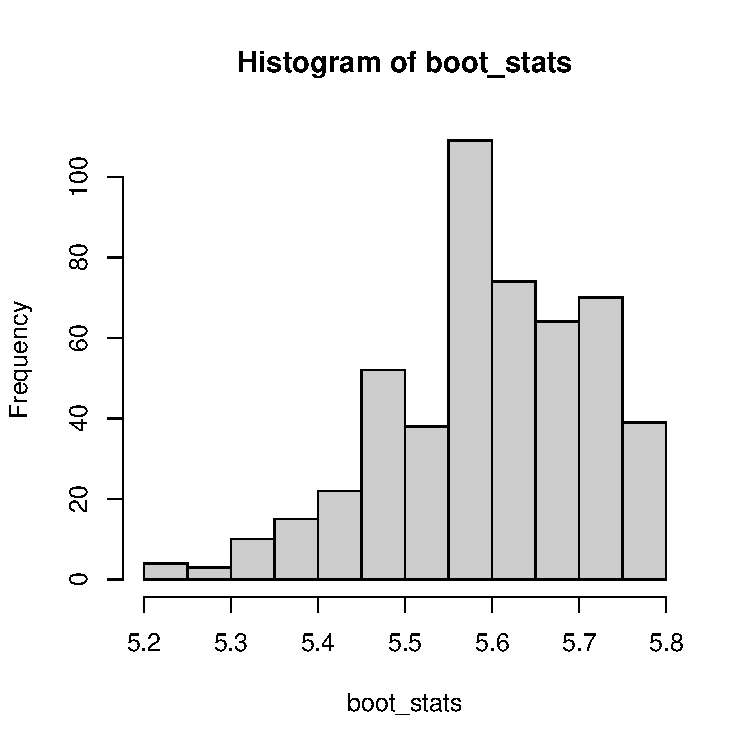
\includegraphics[width=.7\linewidth,height=.7\linewidth]{figure/unnamed-chunk-14-1} 

}



\end{knitrout}

\end{frame}

%------------------------------------------------

\begin{frame}[fragile]
\frametitle{Bootstrap standard error}

The bootstrap standard error is just the standard deviation of the bootstrap samples
\begin{knitrout}\footnotesize
\definecolor{shadecolor}{rgb}{0.969, 0.969, 0.969}\color{fgcolor}\begin{kframe}
\begin{alltt}
\hlcom{# descriptive statistics}
\hlkwd{summary}\hlstd{(boot_stats)}
\end{alltt}
\begin{verbatim}
##    Min. 1st Qu.  Median    Mean 3rd Qu.    Max. 
##    5.20    5.52    5.60    5.60    5.70    5.80
\end{verbatim}
\begin{alltt}
\hlcom{# Bootstrap Standard Error}
\hlkwd{sd}\hlstd{(boot_stats)}
\end{alltt}
\begin{verbatim}
## [1] 0.1167183
\end{verbatim}
\end{kframe}
\end{knitrout}

\end{frame}

%------------------------------------------------

\end{document}
